\documentclass[12pt]{report}
\usepackage[pdftex]{graphicx}
%\usepackage[pdftrex/bookmarksnumbered=true]{hyperref}
\usepackage{hyperref}
\linespread{1.5}
\textwidth = 6in
\textheight = 9in
\usepackage[body={6.0in, 8.2in},left=1.25in,right=1.0in,top=1.0in, bottom=1.0in]{geometry}
\frenchspacing
\usepackage{fancyhdr}
\usepackage{color}
\usepackage{xcolor}
\usepackage{listings}
\usepackage{listings}
\lstset{
language=Java,
basicstyle=\small\sffamily,
numbers=left,
numberstyle=\tiny,
frame=tb,
columns=fullflexible,
showstringspaces=false
}



\usepackage{caption}
\DeclareCaptionFont{white}{\color{white}}
\DeclareCaptionFormat{listing}{\colorbox{gray}{\parbox{\textwidth}{#1#2#3}}}
\captionsetup[lstlisting]{format=listing,labelfont=white,textfont=white}


\begin{document}
\pagenumbering{roman}
%\input{Coverpage.tex}

%----------------title page
%\begin{titlepage}
%\begin{center}
%{\bf \large Graphical Editor in OpenGL}\\
%\vspace{.15in}
%{\bfseries Mini Project Report}\\
%\vspace{.15in}
%{\normalsize Submitted to} \\
%\vspace{.1in}
%{\bfseries DEPARTMENT OF COMPUTER SCIENCE AND ENGINEERING}\\
%\vspace{.25in}
%{\normalsize \emph{By}}\\
%{\bfseries\normalsize Samir Sheriff }\\
%{\bfseries\normalsize Satvik N }\\
%\vspace{.25in}
%{\normalsize \emph{In partial fulfilment of the requirements\\ for the award of the degree \\
%\vspace{.15in}
%} } 
%
%\vspace{.15in}
%{\large{BACHELOR OF ENGINEERING}}\\
%\vspace{.15in}
%{\normalsize{IN}}\\
%\vspace{.15in}
%{\bfseries\normalsize COMPUTER SCIENCE AND ENGINEERING}\\
%\vspace{0.15in}
%
%\begin{figure}[h!]
%	\centering
%		\includegraphics[scale=0.5]{RVCE.png}
%		
%\end{figure} 
%\vspace{.25in}
%{\bfseries\large R V College of Engineering}\\
%{\normalsize (Autonomous Institute, Affiliated to VTU)}\\
%{\bfseries\normalsize BANGALORE - 560059}\\ 
%{\bfseries\large May 2012}
%\end{center}
%\end{titlepage}


%---------Declaration
\begin{titlepage}
%\chapter*{\centerline{DECLARATION}}
\begin{center}
\section*{DECLARATION}
\end{center}

\paragraph{}  We, Samir Sheriff and Satvik N, bearing USN numbers 1RV09CS093 and 1RV09CS095 respectively, hereby declare that the dissertation entitled ``\textbf{Graphical Editor in OpenGL}'', completed and written by us, has not, previously, formed the basis for the award of any degree or diploma or certificate of any other University.
\vspace{1in}

\begin{flushright} {Bangalore \hspace{4.4in} Samir Sheriff } 
 {USN:1RV09CS093}
 \end{flushright}

\begin{flushright} { Satvik N } \\
 {USN:1RV09CS095}
 \end{flushright}
\end{titlepage}
%
%---------Certificate
\begin{titlepage}
\newpage
\begin{center}
{\bfseries\large R V COLLEGE OF ENGINEERING}\\
{\normalsize (Autonomous Institute Affiliated to VTU)}\\
{\normalsize DEPARTMENT OF COMPUTER SCIENCE AND ENGINEERING}\\
\end{center}
	
\begin{figure}[h!]
	\centering
		\includegraphics[scale=0.5]{RVCE.png}
		%\includegraphics{msrit-logo.jpg}
	%\caption{}
	%\label{fig:logo2}
\end{figure}

\begin{center}
\bf{\underline{CERTIFICATE}}
\end{center}
\noindent This is to certify that the dissertation entitled, ``\textbf{Graphical Editor in OpenGL}'',  has been successfully carried out at R.V.C.E., Bangalore
 in partial fulfillment of the requirements for the award of degree 
 in Computer Science and Engineering of Visvesvaraya Technological University, under autonomous scheme, during the academic year 2012-2013.
by  \textbf{Samir Sheriff and Satvik N}  under our supervision and guidance.
\vspace{.5in}

\begin{flushleft} 
 Signature of Lab In-charge  \hspace{4cm} Signature of Lab In-charge \\
 (Mrs. Deepamala N) \hspace{6cm} (Mrs. Jyothi Shetty)\\
\vspace{0.75 in}
\hspace{10cm}
 Signature of HOD	
\\ \hspace{10cm} (Dr. N K. Srinath) \\

 \end{flushleft} 
\begin{flushleft}
\hspace{1in}Name of Examiner \hspace{1.25in} Signature of Examiner
\end{flushleft}
\begin{flushleft}
1: \\
\vspace{.5in} 
2: 
\end{flushleft}
\end{titlepage}


%---------Acknowledgement
  
%\linespread{1.5}
\setcounter{page}{1}
\begin{center}
\section*{ACKNOWLEDGEMENT}
\addcontentsline{toc}{section}{ACKNOWLEDGEMENT}
\end{center}
The euphoria and satisfaction of the completion of the project will be incomplete
without thanking the persons responsible for this venture.


We acknowledge RVCE (Autonomous under VTU) for providing an opportunity to
create a mini-project in the 5th semester. We express our gratitude towards \textbf{Prof. B.S. Satyanarayana}, principal, R.V.C.E for constant encouragement and facilitates extended in completion of this project. We would like to thank \textbf{Prof. N.K.Srinath}, HOD, CSE
Dept. for providing excellent lab facilites for the completion of the project. We would
personally like to thank our project guides \textbf{Mrs. Deepamala N and Mrs. Jyothi Shetty} and also the lab in charge, for providing timely assistance \& guidance at the time.



We are indebted to the co-operation given by the lab administrators and lab assistants,
who have played a major role in bringing out the mini-project in the present form.
Bangalore



\begin{flushright}
Samir Sheriff\\
7th semester, CSE\\
USN:1RV09CS093\\

Satvik N\\
7th semester, CSE\\
USN:1RV09CS095\\

\end{flushright}

\newpage

%--------------Abstract
%\fontfamily{roman}%\selectfont
\begin{center}
\section*{ABSTRACT}
\end{center} 
A Graphics Editor is a feature in any OS that you can use to create drawings on a blank drawing area or in existing pictures. Many of the tools you use in this Graphics Editor are found in the ribbon, which is near the top of the Editor window.


The main objective of the editor is to help the user input graphical data and edit it conveniently. For ease in input and to help the user traverse through the text easily, the editor will provide functionality through the mouse, keyboard, or trackball.



The Graphics Editor in this project has been developed using various algorithm like Mid-point circle drawing algorithm, clipping algorithm, flood-fill Scan-line algorithm, Bezier curves algorithm etc. The editor has been developed in Visual Studio 2010.The various features have been supported by an easy to understand mouse interface. All the tools have been organized under the toolbar.  The color palette has been organized under the color palette. The drawing work is carried out in the sub window which is a part of the main window. The drawing features supported are line, rectangle, ring drawing, Brush, freehand drawing, curve, text, clipping, and eraser.



 This project aims to develop a 2-D Graphics Editor which supports basic operations which include creating objects like lines, circles, polygons,  etc and also transformation operations like translation, scaling, etc on such objects.
 


\addcontentsline{toc}{section}{ABSTRACT}


%------Table Of Contents
\addcontentsline{toc}{section}{CONTENTS}
\tableofcontents
%\listoffigures
%\listoftables


\newpage

\pagenumbering{arabic}
\setcounter{page}{1}

\pagestyle{fancy}
\lhead{\scriptsize{Introduction}}
\chead{}
\rhead{\scriptsize{Graphical Editor in OpenGL}}
\lfoot{\scriptsize{Dept. of CSE, RVCE, Bangalore.}}
\rfoot{\small{\thepage}}
\cfoot{\scriptsize{Sept 2012 - Jan 2013}}
\renewcommand{\headrulewidth}{0.4pt}
\renewcommand{\footrulewidth}{0.4pt}
\chapter{Introduction}
OpenGL is an open specification for an applications program interface for defining 2D and3D objects. The specification is cross-language, cross-platform API for writing applications that produce 2D and 3D computer graphics. It renders 3D objects to the screen, providing the same set of instructions on different computers and graphics adapters. Thus it allows us to write an application that can create the same effects in any operating system using any OpenGL-adhering graphics adapter.



Computer graphics, a 3-dimensional primitive can be anything from a single point to an nsided polygon. From the software standpoint, primitives utilize the basic 3-dimensional rasterization algorithms such as Bresenham's line drawing algorithm, polygon scan line fill, texture mapping and so forth. OpenGL's basic operation is to accept primitives such as points, lines and polygons, and convert them into pixels. This is done by a graphics pipeline known as the OpenGL state machine. Most OpenGL commands either issue primitives to the graphics pipeline, or configure how the pipeline processes these primitives.



OpenGL is a low-level, procedural API, requiring the programmer to dictate the exact steps required to render a scene. OpenGL's low-level design requires programmers to have a good knowledge of the graphics pipeline, but also gives a certain amount of freedom to implement novel rendering algorithms.

\section{Purpose}


The aim of this project is to develop a 2-D graphics package which supports basic operations which include creating objects like lines, circles, polygons, spirals, etc and also transformation operations like translation, scaling, etc on such objects. The package must also have a user-friendly interface that may be menu-oriented, iconic or a combination of both.

\section{Introduction to OpenGl}
OpenGL provides the programmer with an interface to graphics hardware. It is a powerful, low-level rendering and modeling software library, available on all major platforms, with wide hardware support. It is designed for use in any graphics applications, from games to modeling to CAD.



OpenGL intentionally provides only low-level rendering routines, allowing the programmer a great deal of control and flexibility. The provided routines can easily be used to build high-level rendering and modeling libraries, and in fact, the OpenGL Utility Library (GLU), which is included in most OpenGL distributions, does exactly that. Note also that OpenGL is just a graphics library; unlike DirectX, it does not include support for sound, input, networking, or anything else not directly related to graphics.

\subsection{History of OpenGl}
OpenGL was originally developed by Silicon Graphics, Inc. as a multi-purpose, platform independent graphics API. Since 1992, the development of OpenGL has been overseen by the OpenGL Architecture Review Board (ARB), which is made up of major graphics vendors and other industry leaders, currently consisting of ATI, Compaq, Evans \& Sutherland, Hewlett-Packard, IBM, Intel, Intergraph, nVidia, Microsoft, and Silicon Graphics. The role of the ARB is to establish and maintain the OpenGL specification, which dictates which features must be included when one is developing an OpenGL distribution.



Because OpenGL is designed to be used with high-end graphics workstations, it has, until recently, included the power to take full advantage of consumer-level graphics hardware. Furious competition over the last couple of years, however, has brought features once available only on graphics workstations to the consumer level; as a result, there are more and more video cards of which OpenGL can't take full advantage. Eventually, these extensions may become official additions to the OpenGL standard. OpenGL 1.2 was the first version to contain support for features specifically requested by game developers (such as multitexturing), and it is likely that future releases will be influenced by gaming as well.


\subsection{OpenGL Architecture}

OpenGL is a collection of several hundred functions providing access to all the features offered by your graphics hardware. Internally, it acts as a state machine--a collection of states that tell OpenGL what to do. Using the API, you can set various aspects of the state machine, including such things as the current color, lighting, blending, and so on. When rendering, everything drawn is affected by the current settings of the state machine. It's important to be aware of what the various states are, and the effect they have, because it's not uncommon to have unexpected results due to having one or more states set incorrectly.

\begin{figure}[h!]
	\centering
		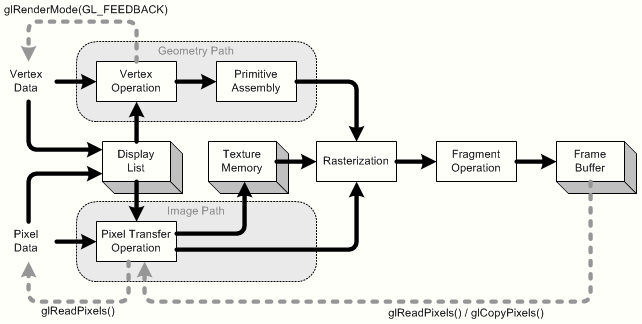
\includegraphics[scale=0.75]{opengl_pipeline.png}
	\caption{The OpenGL Graphics rendering pipeline.}
	\label{fig:logo2}
\end{figure}



At the core of OpenGL is the rendering pipeline, as shown in Figure 2.1. You don't need to
understand everything that happens in the pipeline at this point, but you should at least be aware
that what you see on the screen results from a series of steps. Fortunately, OpenGL handles most of these steps for you.


Under Windows, OpenGL provides an alternative to using the Graphics Device Interface (GDI). GDI architects designed it to make the graphics hardware entirely invisible to Windows programmers. This provides layers of abstraction that help programmers avoid dealing with device-specific issues.


\section{Significance of OpenGL}
\begin{itemize}
\item{With different 3D accelerators, by presenting the programmer To hide the complexities of interfacing with a single, uniform API.}
\item{To hide the differing capabilities of hardware platforms, by requiring that all implementations support the full OpenGL feature set (using software emulation if necessary).}
\item{OpenGL is a well documented API.}
\item{OpenGL is also a clean API and much easier to learn and program.}
\item{OpenGL has the best demonstrated 3D performance for any API.}
\item{OpenGL has a conformance suite to validate that OpenGL implementations correctly implement OpenGL.}
\end{itemize}


\section{Design Aspects of Project in OpenGL}
The Graphics Package is designed using the in built graphics library. The objects, which can be drawn using the editor, are stored as functions that can be used according to the requirements.



We can say that based on the design philosophy used during their implementation, the graphics editors can be of two main types:



One is an Object oriented editor where in each thing drawn in the view port is an object. Such objects can be selected individually and can be subjected to any of the transformations provided in the editor. The advantage of such editors is that the code can be easily written in using an Object Oriented Programming language like C++. Also undo functionalities can be easily implemented because all that the editor has to do is to keep a stack of objects being drawn on the screen. The disadvantage is that the user can only select objects and not a part of the screen.



The other kind of an editor is a pixel-based editor where in drawing anything on the view port is like painting on a canvas. Once an object is drawn it cannot be individually selected. Instead only a rectangular portion of the screen can be usually selected and subjected to various transformations or other operations. In other words the smallest object that can be selected and modified is a pixel. The basic advantage is that of the simplicity in code of such an editor where in the smallest unit is a pixel. The disadvantage being that an individual object cannot be selected and subjected to transformations.



Given the advantages and disadvantages of the two ways of implementing, the programmer is free to choose one that is more appealing to him .The end product needs to be a user-friendly interface. Ease of understanding and speed of working are two main requirements for it, which should be kept in mind during each phase of design and implementation.


\begin{figure}[h!]
	\centering
		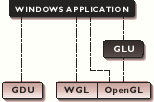
\includegraphics[scale=1.0]{opengl_lib.png}
	\caption{OpenGL API hierarchy under Windows system.}
	\label{fig:logo2}
\end{figure}

 However, GDI is intended for use with applications and thus lacks the speed required for games. OpenGL allows you to bypass GDI entirely and deal directly with graphics hardware. Figure 2.2 illustrates the OpenGL hierarchy under Windows. 

\pagestyle{fancy}
\lhead{\scriptsize{Software Requirements Specification}}
\chead{}
\rhead{\scriptsize{Graphical Editor in OpenGL}}
\lfoot{\scriptsize{Dept. of CSE, R V C E, Bangalore.}}
\rfoot{\small{\thepage}}
\cfoot{\scriptsize{Sept 2012 - Jan 2013}}
\renewcommand{\headrulewidth}{0.4pt}
\renewcommand{\footrulewidth}{0.4pt}

\chapter{REQUIREMENT SPECIFICATION}
Software Requirement Specification (SRS) is an important part of the  software development process. We describe the overall description of the Mini-Project, the specific requirements of the Mini-Project, the software requirements and hardware requirements and the functionality of the system.
\section{Overall Description}
\subsection{Product Perspective}

This is a graphics editor that enables the user to input graphical data.  Using the editor, the user can also save the information input by him/her into files or open existing files for editing.  This editor provides a graphical user - friendly interface to create and edit the files. 

\subsection{Product Functions}

As mentioned previously, the main objective of the editor is to help the user to input graphical data and edit it conveniently. For ease in input and to help the user to traverse through the text easily, the editor provides functionality through the mouse. 

\subsection{User Characteristics}

The editor provides a very easy-to-use interface and does not expect any extra technical knowledge from the user. A basic understanding of all the options provided in the editor would facilitate him in using the editor to the best possible extent. Since it is a mouse-driven interface it is sufficiently easy for any kind of end user to run it. 

\section{Specific Requirement}


\subsection{Software Requirements}

\begin{itemize}
\item{}	Operating system: Microsoft Windows 8 / Ubuntu 12.10 / Mac OS X (Mountain Lion)
\item{}	A Visual C/C++ compiler is required for compiling the source code to make the executable file which can then be directly executed.
\item{}	A built in graphics library like glut and glut32, and header file like glut.h and also dynamic link libraries like glut and glut32 are required.
\end{itemize}
\subsection{Hardware Requirements}
The hardware requirements are very minimal and the software can run on most of the machines. 
\begin{itemize}
\item{}	Processor: Intel Core i7 Extreme Edition or higher
\item{}	Processor Speed - 500 MHz or above 
\item{}	RAM: 8 GB or more
\item{}	Graphics Card: Any card that supports a resolution of 1920 x 1080 or higher, with more than 3540 million transistors
\item{} Hard disk: 7 TB or more

\end{itemize}



\pagestyle{fancy}
\lhead{\scriptsize{Detailed Design}}
\chead{}
\rhead{\scriptsize{Graphical Editor in OpenGL}}
\lfoot{\scriptsize{Dept. of CSE, RVCE, Bangalore.}}
\rfoot{\small{\thepage}}
\cfoot{\scriptsize{Sept 2012 - Jan 2013}}
\renewcommand{\headrulewidth}{0.4pt}
\renewcommand{\footrulewidth}{0.4pt}
\chapter{Detailed Design}

\begin{figure}[h!]
	\centering
		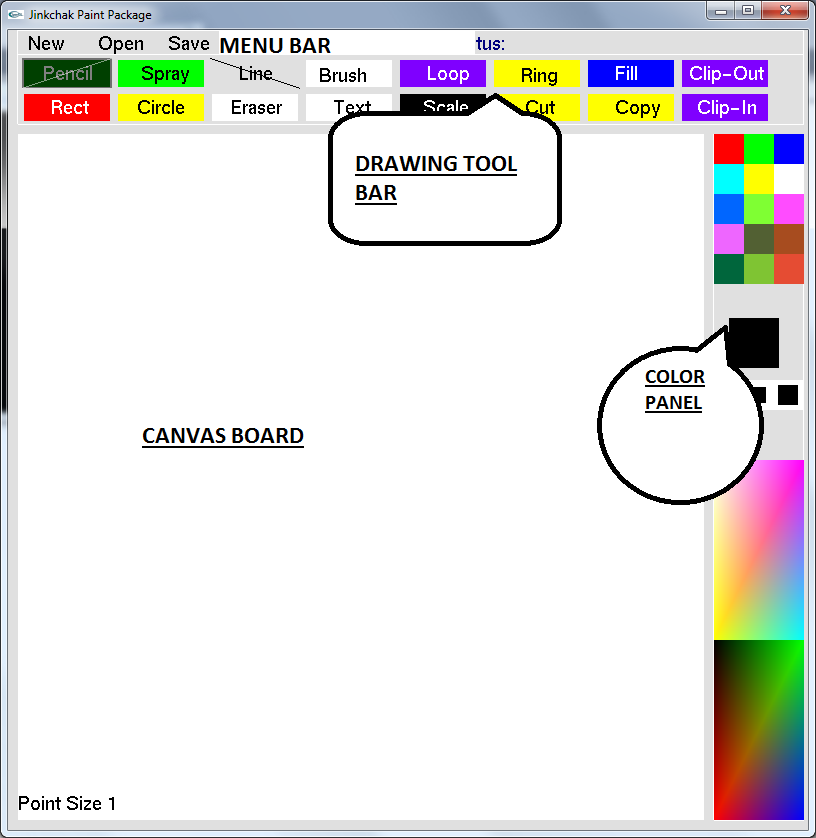
\includegraphics[scale=0.6]{./screenshots/screen_labeling.png}
		%\includegraphics{}
	%\caption{}
	%\label{fig:logo2}
\end{figure}



\section{Object Oriented Class Design}

Object-oriented programming (OOP) is a programming paradigm that represents con-
cepts as "objects" that have data fields (attributes that describe the object) and associated
procedures known as methods. Objects, which are instances of classes, are used to inter-
act with one another to design applications and computer programs.

Had it not been for the presence of the OOP paradigm, our efforts in this project would
have gone in vain, and we do not use that term lightly. Code management was a whole
lot easier when compared to our past experience with procedural programming. In this
chapter, we describe the different classes that were created by us to efficiently manage
our code.

\begin{figure}[h!]
	\centering
		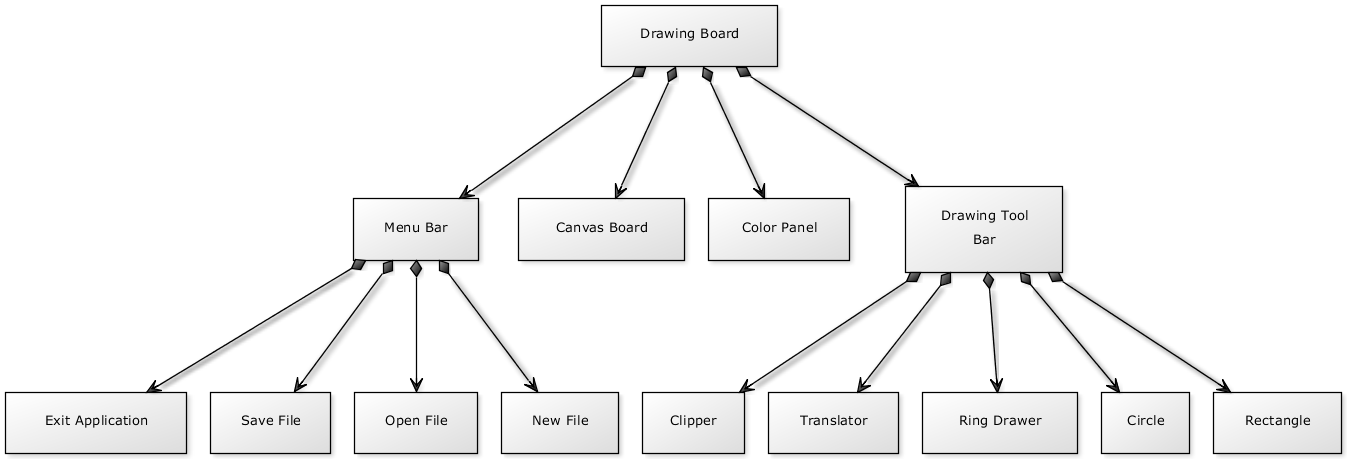
\includegraphics[scale=0.4]{classdesign.png}
		%\includegraphics{}
	%\caption{}
	%\label{fig:logo2}
\end{figure}

\subsection{DrawingBoard Class}

The editor consists of a Drawing Board which, in turn, consists of a color panel on the right, a menu bar and a drawing tool bar on top, and a canvas occupying the rest of the window. Each part of the drawing board is discussed in the sections that follow.



This is the main drawing board class that contains an object of other classes - DrawingToolBar , Color Panel, MenuBar. This class contains some very important methods:

\begin{itemize}
\item{\textbf{initBoard()} - To initialize the board. This method draws all the application window contents - Menubar, Color Panel, Canvas etc.}
\item{\textbf{handlKeyPress()} - To handle the user key presses on the keyboard}
\item{\textbf{handleMouseClick() }- To handle the mouse click}
\item{\textbf{handleMouseClickMotion()} - To handle the mouse click motion} event.
\end{itemize}
The DrawingBoard class only checks in which part of the window a mouse or keyboard event has occurred, and passes control of the program to the respective object (Eg., if the user clicks inside the color panel, the drawing board decides that the color panel and nothing else should handle the click, and hence, it calls the Color Panel’s click handler



\subsection{DrawingTool Class}


This class manages the toolbar panel below the menu bar. It keeps track of all tools present, and provides methods to check whether the user has clicked anywhere in its vicinity. It also provides a draw method that is called by the display function to refresh the contents of the drawing toolbar, when required by the display function of OpenGL. It also keeps track of the current point size of the OpenGL state machine, and provides methods to increase or decrease its size.

In order to keep track of all the tools in the toolbar and call its respective rendering method when selected, the DrawingTool class makes use of another class called the Tool class. This class is an abstract class from which all other tools are derived through inheritance, as shown in the figure. A derived class should always implement the following two methods:
\begin{itemize}
\item{\textbf{render()} - This defines the appearance of this tool’s button on the Drawing Toolbar}
\item{\textbf{drawOnCanvas()} - This defines how the canvas should be manipulated when this tool is selected by the user.}
\end{itemize}

\begin{figure}[h!]
	\centering
		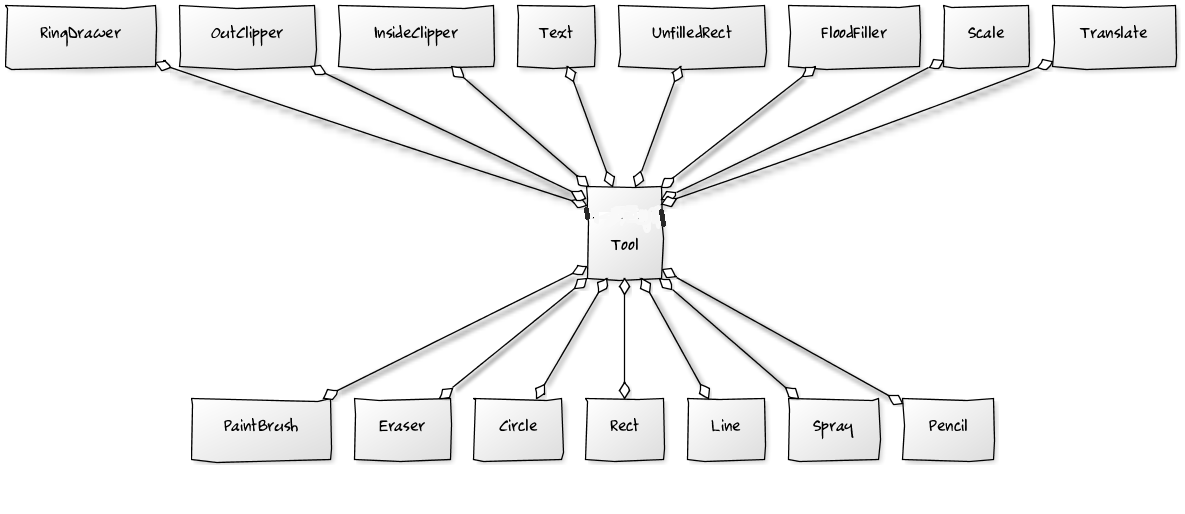
\includegraphics[scale=0.6]{tool.png}
		%\includegraphics{}
	%\caption{}
	%\label{fig:logo2}
\end{figure}


A 2-D array of type “Tool” is maintained, which contains pointers to each tool in the toolbar. The DrawingTool object calls these two methods as an when required. Adding new tools is as easy as creating a new class with the Tool class as the base class, and implementing the two methods mentioned above. No other changes need to be made to any other classes with this design (except in emergencies, due to stupid cyclic dependency errors, which C++ can’t handle, as in the case of the Text Tool).


Here's a description of some of the tools in our editor:

\begin{itemize}
\item{A \textbf{pencil }is a writing implement or art medium usually constructed of a narrow, solid pigment core inside a protective casing. The pencil in our editor allows the user to create free-hand drawings as though he/she were using a real pencil.}
\item{\textbf{Spray }painting is a painting technique where a device sprays a coating (paint, ink, varnish, etc.) through the air onto a surface. The spray in our editor attempts to reproduce this effect virtually.}
\item{The notion of \textbf{line or straight line }was introduced by ancient mathematicians to represent straight objects with negligible width and depth. A line, in our editor, is drawn by selecting two points - a start point and an end point. The start point begins with a mouse click and the end point is the point where mouse button is released.} 
\item{A \textbf{rectangle }is any quadrilateral with four right angles. A user can draw a rectangle, the size of which can be adjusted in real time, by moving the mouse.}
\item{A \textbf{circle }is a simple shape of Euclidean geometry that is the set of all points in a plane that are a given distance from a given point, the centre. A user can draw such a circle, the size of which can be adjusted in real time, by moving the mouse.}
\item{An \textbf{eraser }(US and Canada) or rubber (elsewhere) is an article of stationery that is used for removing pencil markings, and the eraser in our editor does just that. The size of the eraser can be varied, either from the color panel, or by using the \textit{,} or \textit{.} keys.}
\item{The \textbf{ring }tool can be used to draw eccentric circles to create a pseudo-3D effect. For instance, clicking and dragging the mouse pointer in the canvas when this tool is selected, produces a pseudo-cone.}
\item{\textbf{Text} may refer to the representation of written language. In order to use the text tool, the user must first select it from the toolbar. Then, he/she must select the text operator from the Menubar and type out the necessary text using the typewriter. Once done, the enter key should be pressed, and that's it. The user can click the mouse anywhere in the canvas to replicate the text typed. }
\item{The \textbf{scale }ratio of some sort of model which represents an original proportionally is the ratio of a linear dimension of the model to the same dimension of the original. Our editor allows parts of the canvas to be scaled up or down for easy viewing.}
\item{In human-computer interaction, \textbf{cut and paste and copy and paste} are related commands that offer a user-interface interaction technique for transferring pixels from a source to a destination. Our editor allows the user to draw a bounding box around the region that has to be cut/copied. Once done, the user can \textbf{click and drag} anywhere else around the canvas to paste the selection. Once the paste location is decided, the user can release the mouse button.}
\item{The \textbf{fill }tool of our editor determines which parts of the canvas to fill with a color selected from the color panel.}
\item{Any procedure which identifies that portion of a picture which is either inside or outside a region is referred to as \textbf{clipping}. Our editor provides this extremely useful feature.}

\end{itemize}


\subsection{Color Panel Class}
The object of this class represents  the color panel that is present in the right part of the application. This panel consists of the following main sections
\begin{itemize}
\item{\textbf{Basic Color Block Section }}: This section shows the basic color block squares which can be selected by clicking on them.
\item{\textbf{Selected Color Box:}} The selected color either in the basic color block or in the color selection triangle is shown in this color box.
\item{\textbf{Size Selectors :}} This section is used to select the drawing size of the current tool. There are three sizes small, medium, large.
\item{\textbf{Color Blender }}- There are two color blenders based on RGB color model and CMYK color model. A variety of colors can be selected from this section
\end{itemize}



\subsection{MenuBar Class}
In a restaurant , a menu is a presentation of food and beverage offerings. However, you will be pleased to know that the menu in our editor is not like that. Our menu is a list of options or commands presented to an operator by a computer or communications system (the Chicken Curry editor, in our case)



In order to keep track of all the menu operations in the menubar and call its respective rendering method when selected, the \textbf{MenuBar} class makes use of another class called the \textbf{MenuOp} class. This class is an abstract class from which all other menu operations are derived through inheritance, as shown in the figure. A derived class should always implement the following two methods:
\begin{itemize}
\item{}\textbf{render() }- This defines the appearance of this tool\' s button on the Drawing Toolbar
\item{}\textbf{performOperation()} - This defines the operation that should be carried out when this op is clicked
\end{itemize}

\begin{figure}[h!]
\centering
  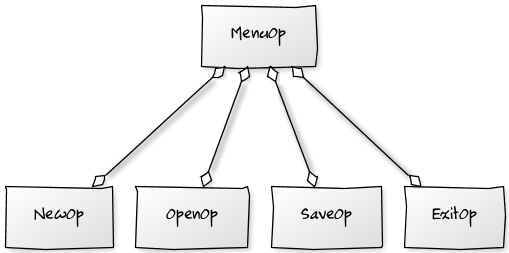
\includegraphics[scale=0.5]{menuop.png}
\caption{Application Window - Start Up Screen}
\end{figure}


The MenuBar object calls these two methods as and when required. Adding new tools is as easy as creating a new class with the \textbf{MenuOp} class as the base class, and implementing the two methods mentioned above. No other changes need to be made to any other classes with this design.


Menu Options supported in the Graphics editor
\begin{itemize}
\item{}\textbf{New} - To create a new canvas used for drawing.
\item{}Open File - To open an already saved canvas drawing file.
\item{}Save File - To save the current canvas drawing to a file.
\item{}Exit application - To exit our Application.
\end{itemize}


When the user clicks the open or save buttons, it ain't a good idea to ask him/her to enter the filename in the console. It would be better for everyone involved, to accept input from the user's keyboard in the editor's window itself. The TypeWriter class was born for this very purpose. It saves the day by offering the following services to the MenuOp class:
\begin{itemize}


\item{It can be started by one operation and requested not to accept more requests until it is done}
\item{While it is buffering input from the user after being turned on, it doesn't accept any more requests, hence, preventing race conditions. It turns on a busy indicator.}
\item{Once done buffering input (when the user presses the enter key), it switches off the busy indicator LED and the requesting party is provided with the contents of the typewriter's buffer to do whatever it feels like with it.}
\item{It writes its output on the right side of the Menu Bar.}

\end{itemize}



\subsection{Canvas Class}

A canvas  is an extremely heavy-duty plain-woven fabric, popularly used by artists as a painting surface, typically stretched across a wooden frame. Our canvas is a virtual representation of such an entity. It allows the user to draw whatever he/she feels like, using the tools and color palette provided.

It contains a 2D array that records every artistic endeavour of the user. It provides methods to save this array to a file so that it can be loaded later. 

What happens if the user finds out that he/she has made a mistake and wants to revert to an older state. Well, say hello to our custom History engine that tracks as many as 30 major updates of the canvas, and allows the user to undo changes, with only a touch of the F2 button. A redo facility, mapped to the F3 key, has also been provided, to head back to the future!





\pagestyle{fancy}
\lhead{\scriptsize{Conclusion}}
\chead{}
\rhead{\scriptsize{Graphical Editor in OpenGL}}
\lfoot{\scriptsize{Dept. of CSE, RVCE, Bangalore.}}
\rfoot{\small{\thepage}}
\cfoot{\scriptsize{Sept 2012 - Jan 2013}}
\renewcommand{\headrulewidth}{0.4pt}
\renewcommand{\footrulewidth}{0.4pt}
\chapter{CONCLUSION AND FUTURE WORK}

\section{Summary}
We would like to give back to this world a state-of-the-art Graphical editor, designed with object-oriented principles so that it can be easily extended (unlike mypackage.cpp) by others who choose to show our project next year. With great power comes great responsibility. This was, is and will always be free and will be used in schools, colleges, universities, Government and Private Institutions, secret services, the mafia, etc. We had wished to release this product before Christmas so that students can enjoy it during the holiday season. and now, our wish has come true.

\section{Limitations}
\begin{itemize}
\item{}The graphics editor doesn't work in full screen.
\item{} The drawn picture cannot be saved as a picture file like png, jpeg. It is saved as  a binary file.
\item{}	There is a lag when using tools like pencil, spray, etc. are used.
\item{}	Three dimensional viewing and editing of pictures are not possible. 
\end{itemize}

\section{Future enhancements}
\begin{itemize}
\item{} This package was developed on Windows 7, and can be made a platform independent application.
\item{}	The drawings can be made to save as pictures and help the user share them in various social networking sites like facebook, google+ etc.
\item{}	This package can be made efficient by exploiting the opengl graphics pipeline system.
\item{}Various special tools like Scan fillers, image enhancing tools can be added.

\end{itemize}

\newpage

%For Bib refer to refs.bib to add/remove bib items
\addcontentsline{toc}{section}{BIBLIOGRAPHY}
\begin{thebibliography}{refs}
\bibitem{test}OpenGL Book - A free online opengl programming book.  -\url{http://openglbook.com/}
\bibitem{t}OpenGL - Wikipedia, the free encyclopedia - \url{http://en.wikipedia.org/wiki/OpenGL}
%\bibtitem{te}Decision Trees - \url{http://web.cecs.pdx.edu/~mm/MachineLearningWinter2010/pdfslides/DecisionTrees.pdf}
\bibitem{t} OpenGL Programming Guide  - \url{https://www.glprogramming.com/red/}
\bibitem{t}OpenGL SuperBible - \url{http://www.starstonesoftware.com/OpenGL/}
\bibitem{t} Opengl Graphics Editor in Google Code- \url{http://code.google.com/p/opengl-graphics-editor/}
\bibitem{t}Opengl on github - \url{https://github.com/samiriff/GraphicalEditor}

%\bibitem{}
%\bibitem{}
\end{thebibliography}

\newpage
\pagestyle{fancy}
\lhead{\scriptsize{Appendix A: Source Code}}
\chead{}
\rhead{\scriptsize{Graphical Editor in OpenGL}}
\lfoot{\scriptsize{Dept. of CSE, RVCE, Bangalore.}}
\rfoot{\small{\thepage}}
\cfoot{\scriptsize{Sept 2012 - Jan 2013}}
\renewcommand{\headrulewidth}{0.4pt}
\renewcommand{\footrulewidth}{0.4pt}

\addcontentsline{toc}{section*}{APPENDICES}
\section*{Appendices}
\section*{Appendix A : Source Code}


\lstinputlisting[ language=C++, breaklines=true]{DrawingBoard.h}


%
%\lstinputlisting[language=C++, label=huffman,caption=The definition  of the class Huffman\, this class helps in building the huffman tree for an input file.]{HuffmanCode.h}
%
%\lstinputlisting[language=C++, label=compresswrite,caption=The definition  of the class CompressionWriting\, this class helps in writing the bits to the compressed file.]{CompressionWriting.h}
%
%\lstinputlisting[language=C++, label=huff,caption=The main program of the huffman compression algorithm.]{huff.cpp}
%
%\lstinputlisting[language=C++, label=unhuff,caption=The definition of the class Decompressor\, this class helps in decompressing the compressed file using huffman algorithm.]{Decompressor.h}
%
%\lstinputlisting[language=C++, label=unhuff,caption=The main program of the huffman decompression algorithm.]{unhuff.cpp}


%\lstinputlisting[language=C++, label=unhuff,caption=The definition of the class TCP\_Server\, an object of this class is a server object that can concurrently handle requests for files from the clients.]{TCP_Server.h}

%\lstinputlisting[language=C++, label=unhuff,caption=The definition of the class TCP\_Client\, an object of this class indicates a client object that can request for files from the server.]{TCP_Client.h}


\newpage
\pagestyle{fancy}
\lhead{\scriptsize{Appendix B: Screen shots}}
\chead{}
\rhead{\scriptsize{Graphical Editor in OpenGL}}
\lfoot{\scriptsize{Dept. of CSE, RVCE, Bangalore.}}
\rfoot{\small{\thepage}}
\cfoot{\scriptsize{Sept 2012 - Jan 2013}}
\renewcommand{\headrulewidth}{0.4pt}
\renewcommand{\footrulewidth}{0.4pt}


\section*{Appendix B : Screen Shots}
\begin{figure}[h!]

  \centering
    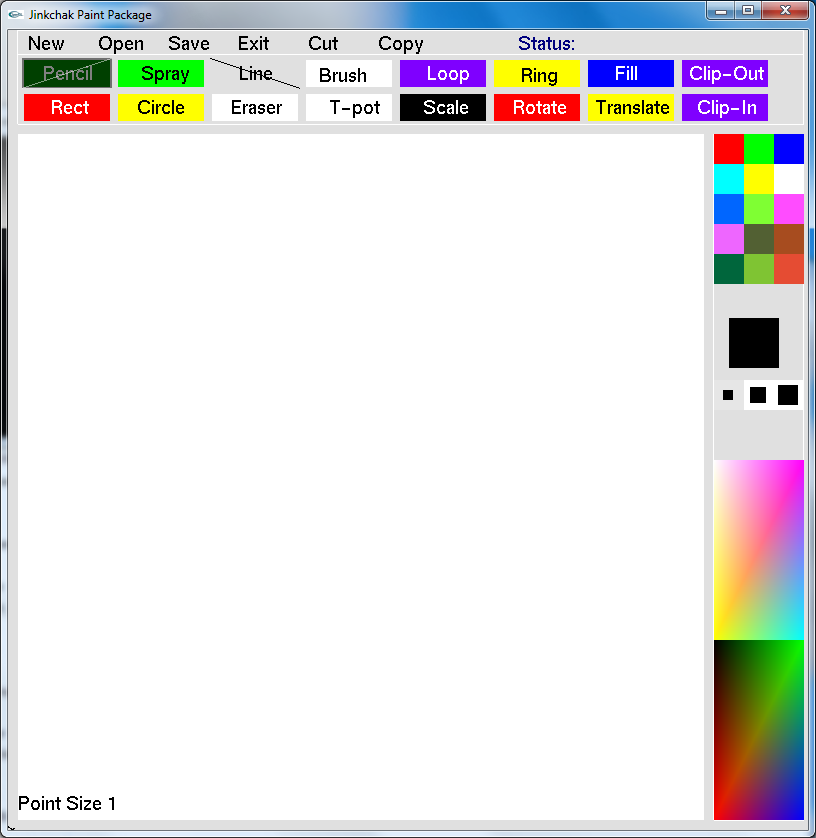
\includegraphics[scale=0.361]{screenshots/init_screen.png}
  \caption{Application Window - Start Up Screen}
\end{figure}

\begin{figure}[h!]

  \centering
    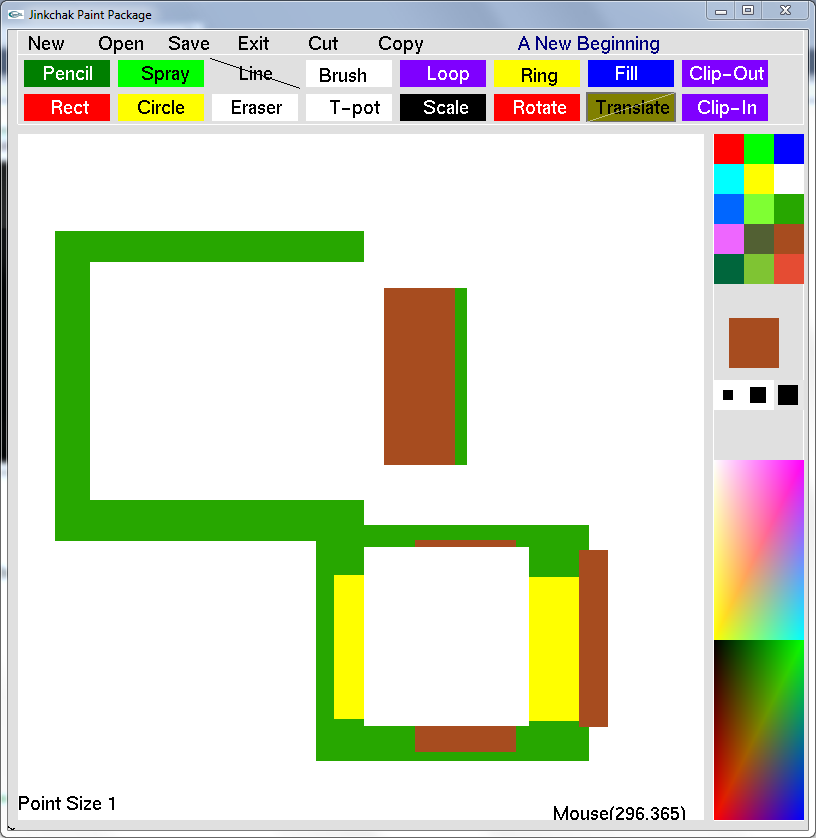
\includegraphics[scale=0.45]{screenshots/translate_demo.png}
  \caption{Translating a portion of a drawing using the Translate tool.}
\end{figure}


\begin{figure}[h!]  
  \centering
    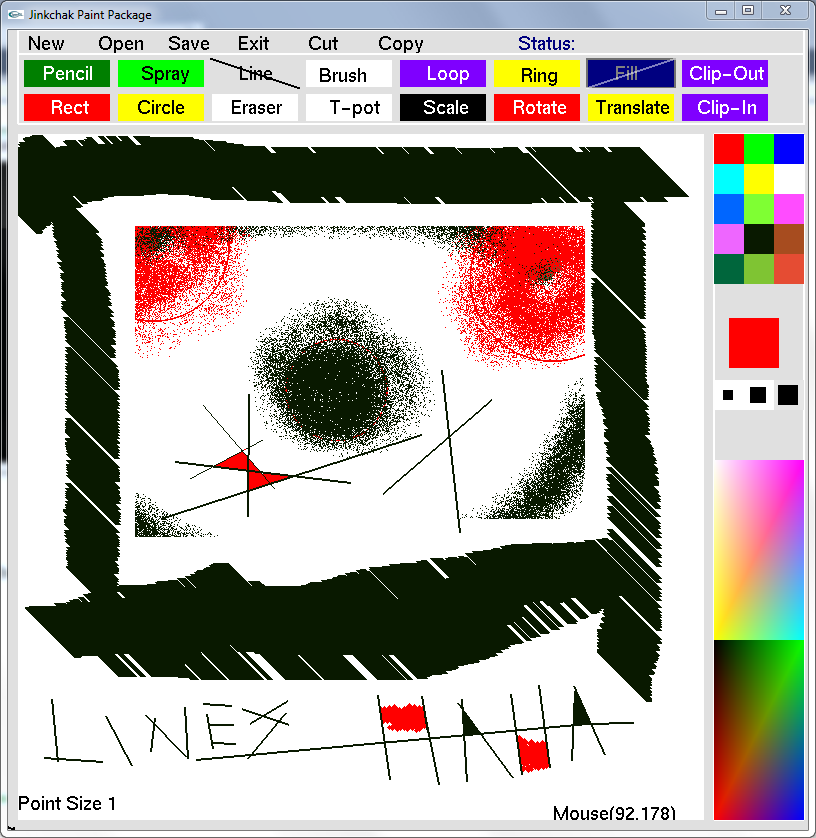
\includegraphics[scale=0.45]{screenshots/lines.png}
\caption{Drawing on the canvas with lines.}
\end{figure}

\begin{figure}[h!]
  
  \centering
    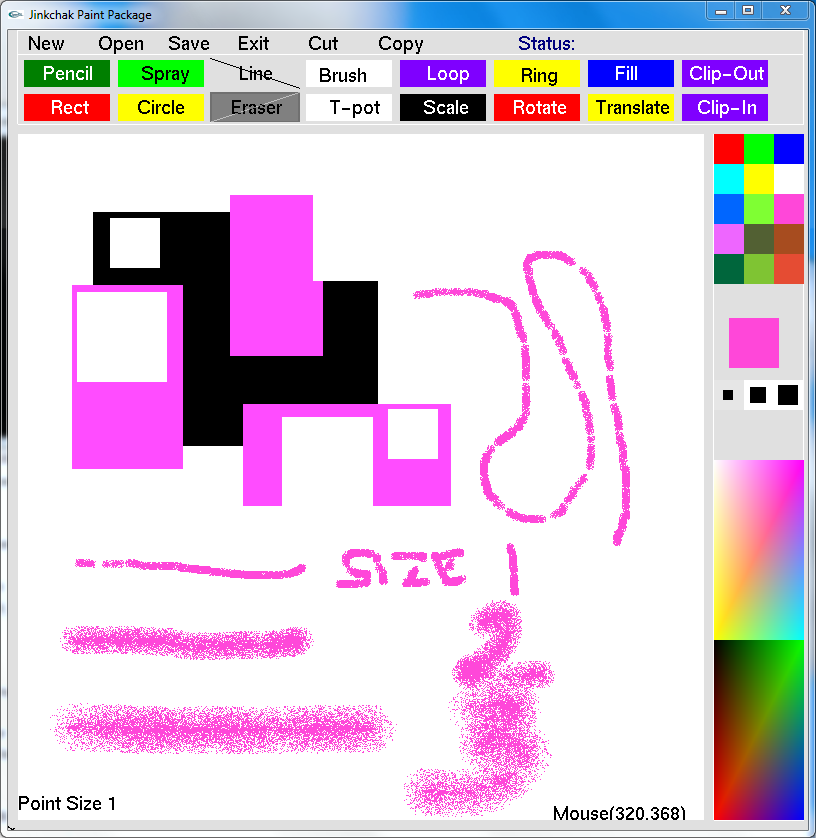
\includegraphics[scale=0.45]{screenshots/rectangle_spray.png}
\caption{Drawing the rectangles and spraying the colors.}
\end{figure}
\begin{figure}[h!]
  
  \centering
    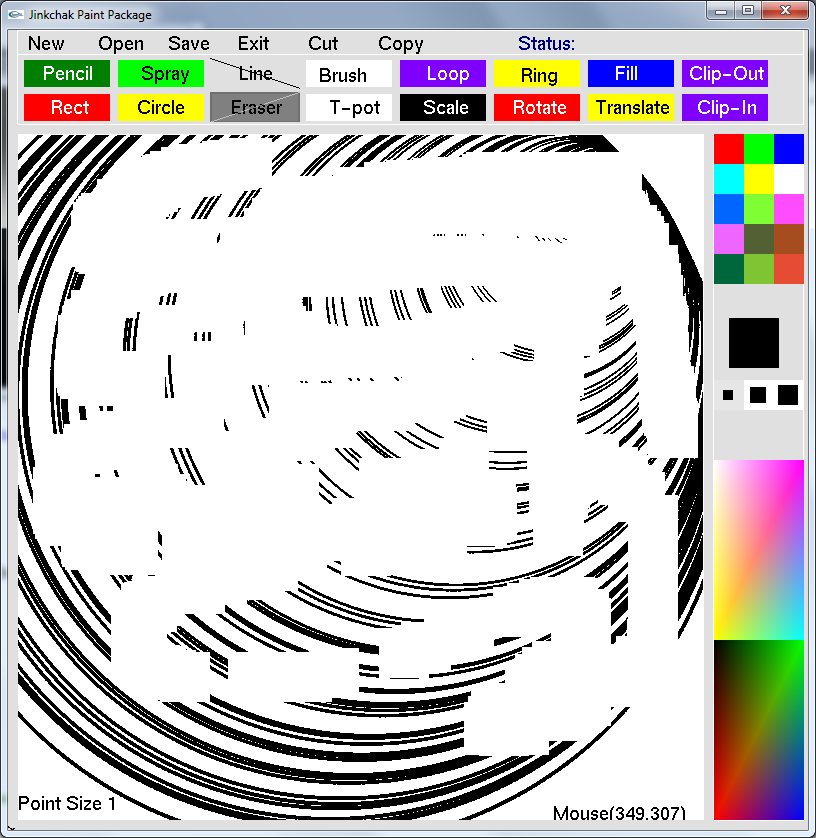
\includegraphics[scale=0.45]{screenshots/eraser.png}
\caption{Erasing the drawing with the eraser.}
\end{figure}
\begin{figure}[h!]
  
  \centering
    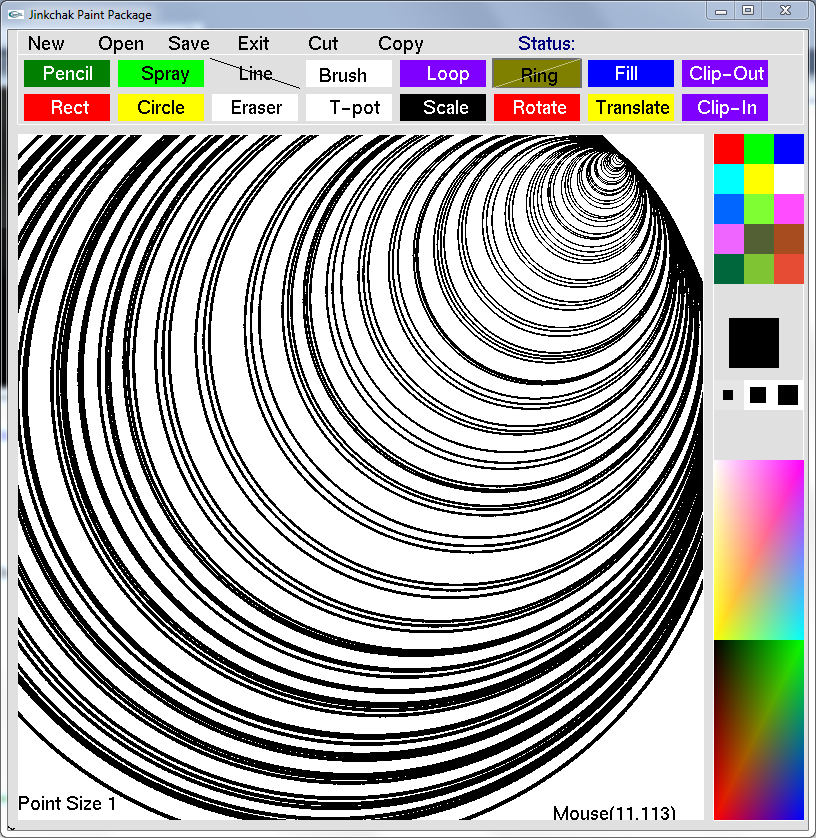
\includegraphics[scale=0.45]{screenshots/ring_pattern.png}
\caption{Ring Pattern - Drawn with the ring drawer special tool.}
\end{figure}

\begin{figure}[h!]
  
  \centering
    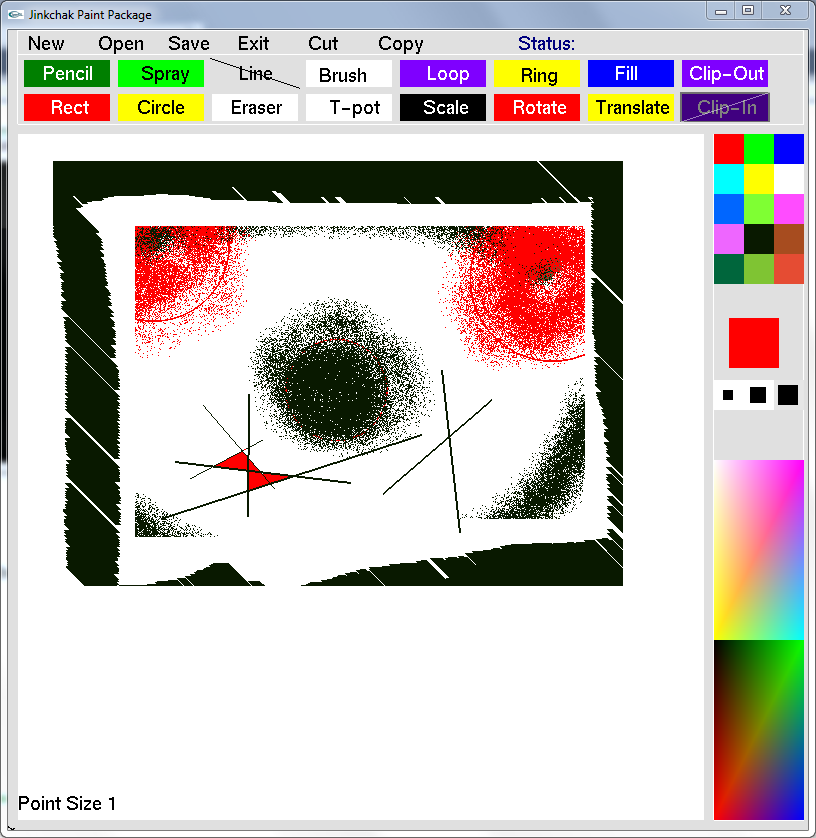
\includegraphics[scale=0.45]{screenshots/inside_clip.png}
\caption{Inside Clipping with the inside clipper tool.}
\end{figure}

\begin{figure}[h!]
  
  \centering
    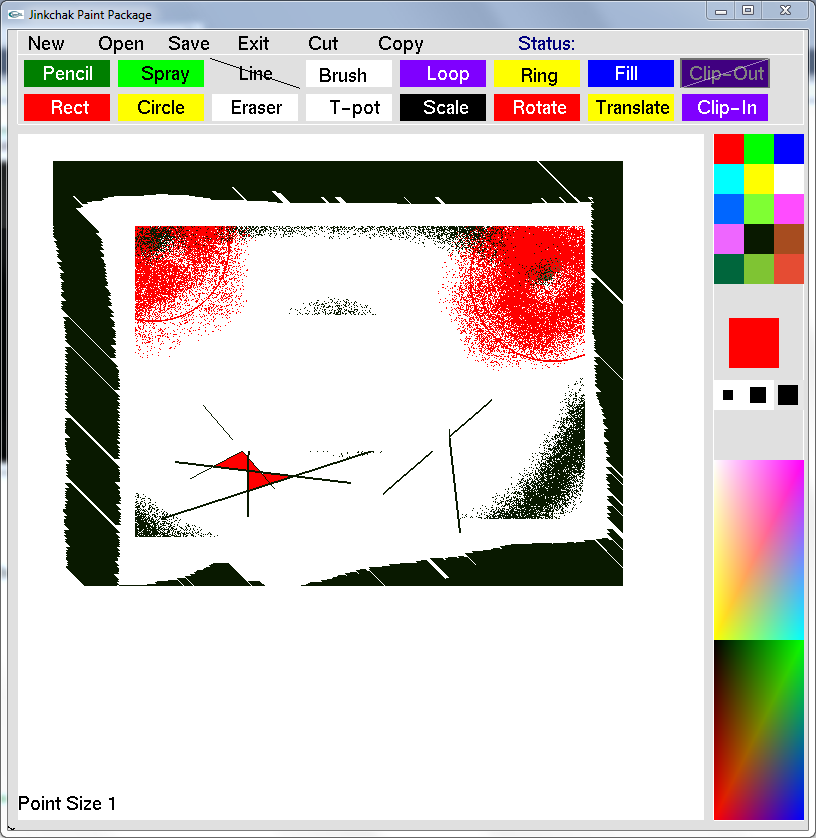
\includegraphics[scale=0.45]{screenshots/out_side_clip.png}
\caption{Outside clipping with the outside clipper tool.}
\end{figure}

\begin{figure}[h!]
  
  \centering
    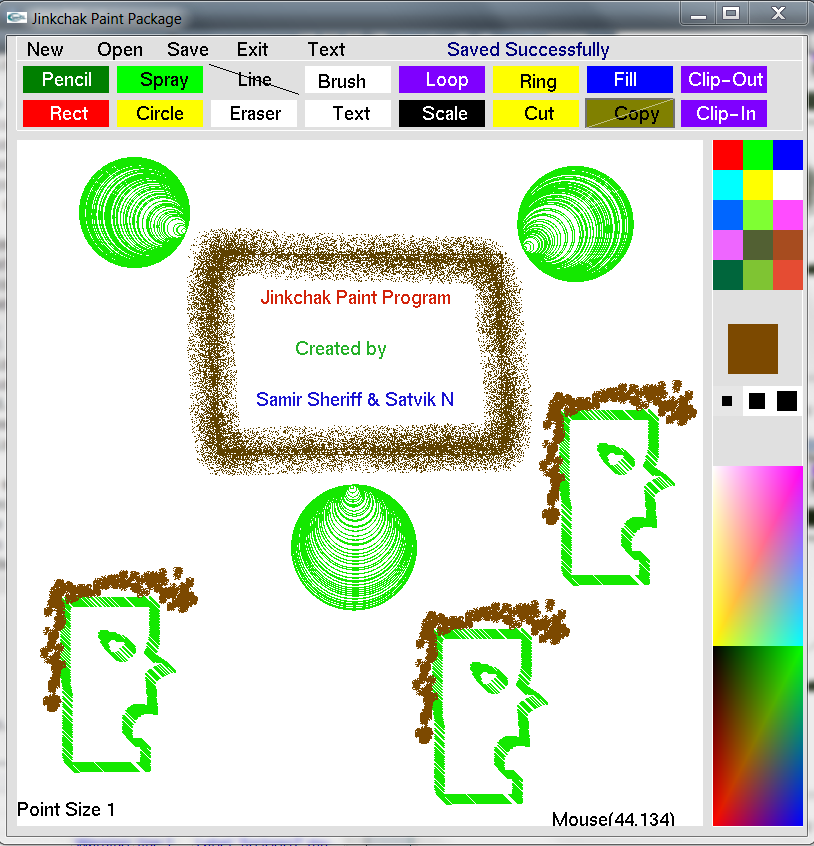
\includegraphics[scale=0.9]{screenshots/CreatedBy.png}
\caption{Image created in its entirety by our Editor}
\end{figure}


\end{document}
